%!TEX program = xelatex

\documentclass[UTF8]{ctexart}
\usepackage{ctex}

\CTEXsetup[format={\Large\bfseries}]{section}

\usepackage[version=3]{mhchem} % Package for chemical equation typesetting
\usepackage{siunitx} % Provides the \SI{}{} and \si{} command for typesetting SI units
\usepackage{graphicx} % Required for the inclusion of images
\graphicspath{{assets/}}
\usepackage{natbib} % Required to change bibliography style to APA
\usepackage{amsmath} % Required for some math elements 
\usepackage{amssymb}
\usepackage[hidelinks]{hyperref}
\usepackage{makecell} % 3 Packages for flexible tabular
\usepackage{multirow}
\usepackage{multicol}

\usepackage{pdfpages}  % include pdf pages for original data etc.

\usepackage{geometry}% 版面大小
\geometry{a4paper,scale=0.7}

\usepackage{fontspec}

\setCJKfamilyfont{hwxk}{STXingkai}% 字体
\newcommand{\hwxk}{\CJKfamily{hwxk}}

\usepackage{fancyhdr}% 页眉页脚
\fancypagestyle{EE_Digital1Exp_template}{
    \fancyhead[L]{\Large {\hwxk 南京大学电子科学与工程学院}}
    \fancyhead[R]{数字系统1实验报告}
    \fancyfoot[c]{- \thepage \ -}
    \renewcommand\footrulewidth{0pt}
}

% 4级目录
\setcounter{secnumdepth}{4}
\setcounter{tocdepth}{4}

\usepackage{graphicx} % Packages for figures
\usepackage{caption2}
\usepackage{subfigure}
\usepackage{float}

\usepackage{listings} % Packages for code block
\usepackage{xcolor}

% for verilog code coloring
\definecolor{vgreen}{RGB}{104,180,104}
\definecolor{vblue}{RGB}{49,49,255}
\definecolor{vorange}{RGB}{255,143,102}

\lstdefinestyle{verilog-style}
{
    language=Verilog,
    basicstyle=\small\ttfamily,
    keywordstyle=\color{vblue},
    identifierstyle=\color{black},
    commentstyle=\color{vgreen},
    numbers=left,
    numberstyle=\tiny\color{black},
    numbersep=10pt,
    tabsize=8,
    moredelim=*[s][\colorIndex]{[}{]},
    literate=*{:}{:}1
}

\makeatletter
\newcommand*\@lbracket{[}
\newcommand*\@rbracket{]}
\newcommand*\@colon{:}
\newcommand*\colorIndex{%
    \edef\@temp{\the\lst@token}%
    \ifx\@temp\@lbracket \color{black}%
    \else\ifx\@temp\@rbracket \color{black}%
    \else\ifx\@temp\@colon \color{black}%
    \else \color{vorange}%
    \fi\fi\fi
}
\makeatother

\usepackage{trace}




%设置图片、表格编号
\renewcommand{\thetable}{\thesubsection{}-\arabic{table}}
\renewcommand{\thefigure}{\thesubsection{}-\arabic{figure}}
\renewcommand{\thefigure}{\thesubsection{}-\arabic{equation}}
\usepackage{amsmath}
\numberwithin{figure}{subsection}
\numberwithin{table}{subsection}
\numberwithin{equation}{subsection}

\setlength\parindent{6pt} % Removes all indentation from paragraphs

\renewcommand{\labelenumi}{\alph{enumi}.} % Make numbering in the enumerate environment by letter rather than number (e.g. section 6)

%\usepackage{times} % Uncomment to use the Times New Roman font

%----------------------------------------------------------------------------------------
%	DOCUMENT INFORMATION
%----------------------------------------------------------------------------------------

\title{\textbf{实验五\ 抢答电路}} % Title

\author{电子科学与工程学院\ 刘时宜\ 201180078} % Author name

\date{} % Date for the report

\begin{document}

\pagestyle{EE_Digital1Exp_template}

\maketitle % Insert the title, author and date

\begin{center}
    \begin{tabular}{l r}
    实验日期: & 2021年12月15日 \\ % Date the experiment was performed
             & 2021年12月22日 \\ % Date the experiment was performed
    指导老师: & 高健 % Instructor/supervisor
    \end{tabular}
    \par 点击目录、书签栏、以及行文中的图表标号的均可跳转至相应页面
    \end{center}
    
% If you wish to include an abstract, uncomment the lines below
% \begin{abstract}
% Abstract text
% \end{abstract}

\tableofcontents

\section{实验目的}
\begin{enumerate}
    \item 利用555芯片搭建单稳态电路
    \item 利用单稳态电路搭建定时抢答电路
\end{enumerate}

\section{实验仪器与主要器材}
\begin{center}
    \begin{tabular}{ll}
        \textbf{仪器:} & \\
        KEYSIGHT DSOX1102AG 示波器 & 1台\\
        示波器高频探头 & 1套\\
        ROGOL DM3068 万用表 & 1台\\
        \textbf{软件:} & \\
        Multisim & 14.1 \\
        \textbf{芯片:} & \\
        74LS74 & 1片 \\
        74HC11 & 1片 \\
        555定时器 & 1片 \\
        \textbf{电路材料:} & \\
        按键开关 & 4个 \\
        发光二极管 & 4个 \\
        电阻 & 若干 \\
        导线 & 若干 \\
    \end{tabular}
\end{center}

\section{实验原理}
\par 555定时器是一种集成电路芯片,常被用于定时器、脉冲产生器和振荡电路。555可被作为电路中的延时器件、触发器或起振元件。
\par 555定时器可工作在三种工作模式下:
\begin{enumerate}
    \item 单稳态模式:在此模式下,555功能为单次触发。应用范围包括定时器,脉冲丢失检测,反弹跳开关,轻触开关,分频器,电容测量,脉冲宽度调制(PWM)等。
    \item 无稳态模式:在此模式下,555以振荡器的方式工作。这一工作模式下的555芯片常被用于频闪灯、脉冲发生器、逻辑电路时钟、音调发生器、脉冲位置调制(PPM)等电路中。如果使用热敏电阻作为定时电阻,555可构成温度传感器,其输出信号的频率由温度决定。
    \item 双稳态模式(或称施密特触发器模式):在DIS引脚空置且不外接电容的情况下,555的工作方式类似于一个RS触发器,可用于构成锁存开关。
\end{enumerate}
\par 利用555定时器搭建单稳态触发器,即可利用单稳态触发器输出信号以及其他逻辑电路构成定时抢答电路。

\section{实验过程}
\subsection{555定时器搭建单稳态触发器}
\subsubsection{原理电路}
\par 实验电路原理图如\ref{monostable sim cir}所示,构成单稳态触发电路,TRI端低电平脉冲时触发输出高电平脉冲。对电路进行仿真,仿真结果如图\ref{monostable sim res}所示。

\begin{figure}[H]
    \begin{center}
        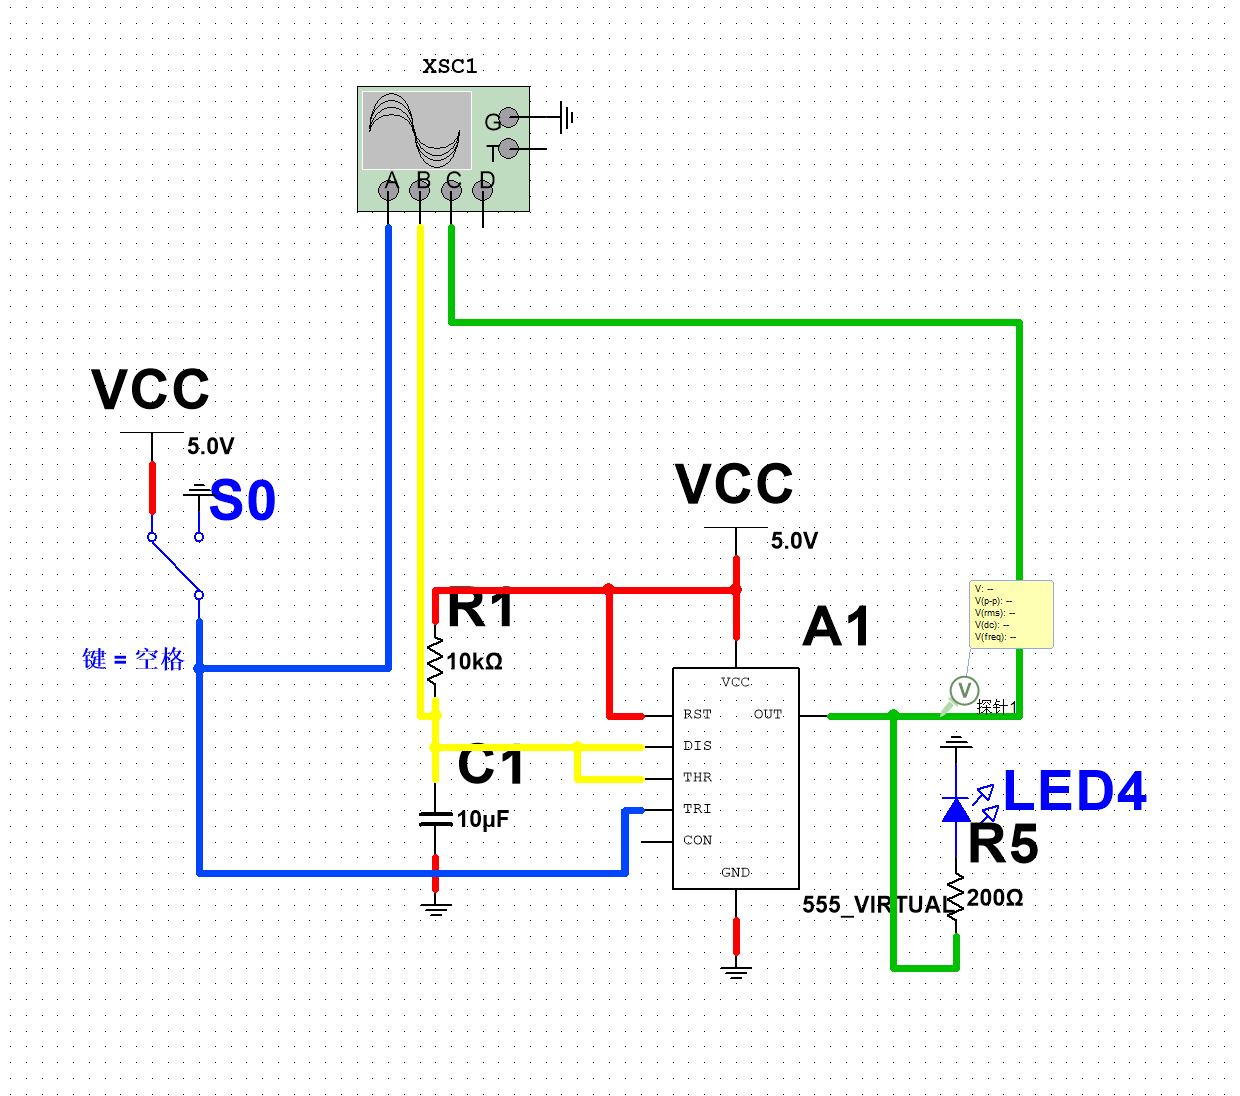
\includegraphics[width=0.8\textwidth]{555/monostable/sim circuit.png}
    \end{center}
    \caption{555单稳态触发器:原理电路}
    \label{monostable sim cir}
\end{figure}

\begin{figure}[H]
    \begin{center}
        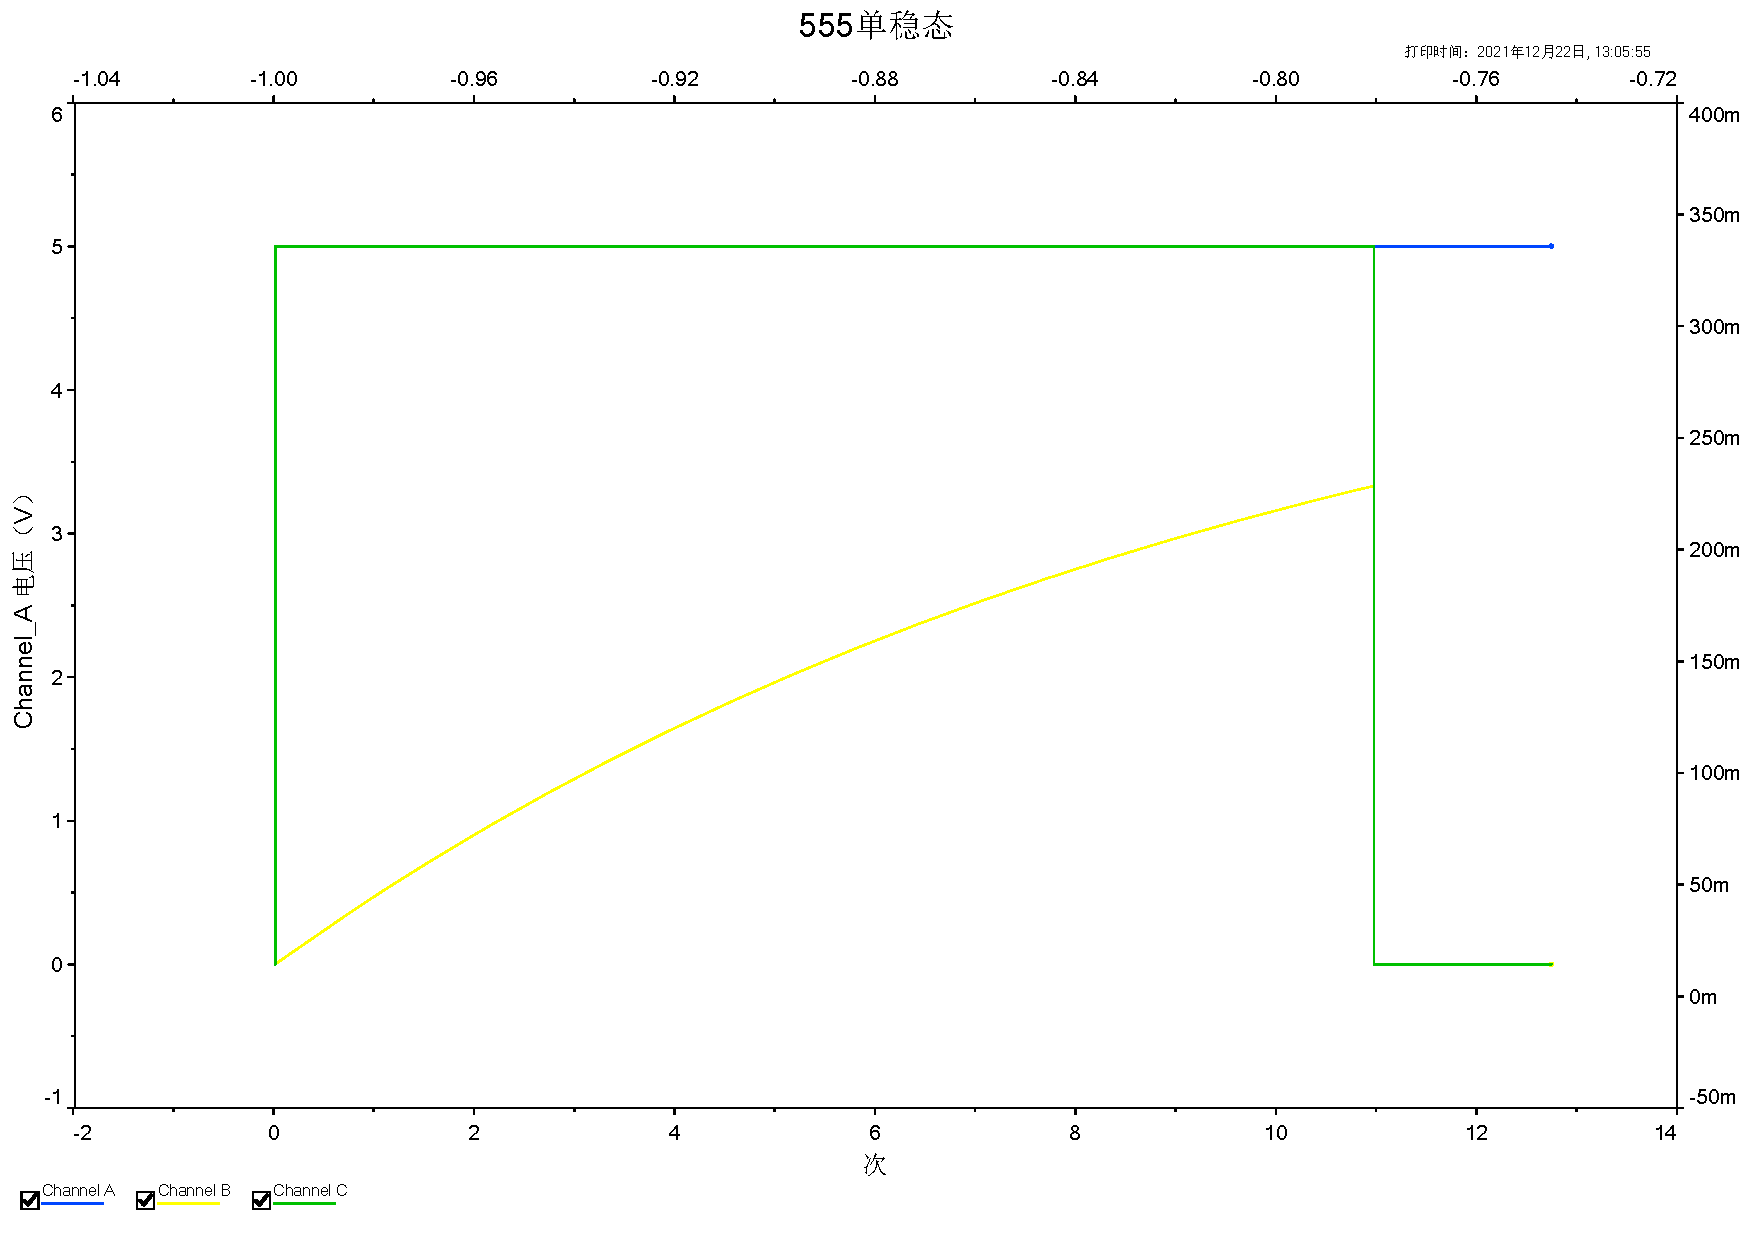
\includegraphics[width=0.8\textwidth]{555/monostable/sim result.pdf}
    \end{center}
    \caption{555单稳态触发器:仿真波形}
    \label{monostable sim res}
\end{figure}

\subsubsection{实验验证}
\par 按照原理电路中的电路连接、元件参数搭建实验电路,实验电路如图\ref{monostable exp cir}所示。其中触发端TRI接信号发生器信号,信号参数为:高电平\SI{5}{\volt},低电平\SI{0}{\volt},周期\SI{200}{\micro\second},高电平占空比80\%。

\begin{figure}[H]
    \begin{center}
        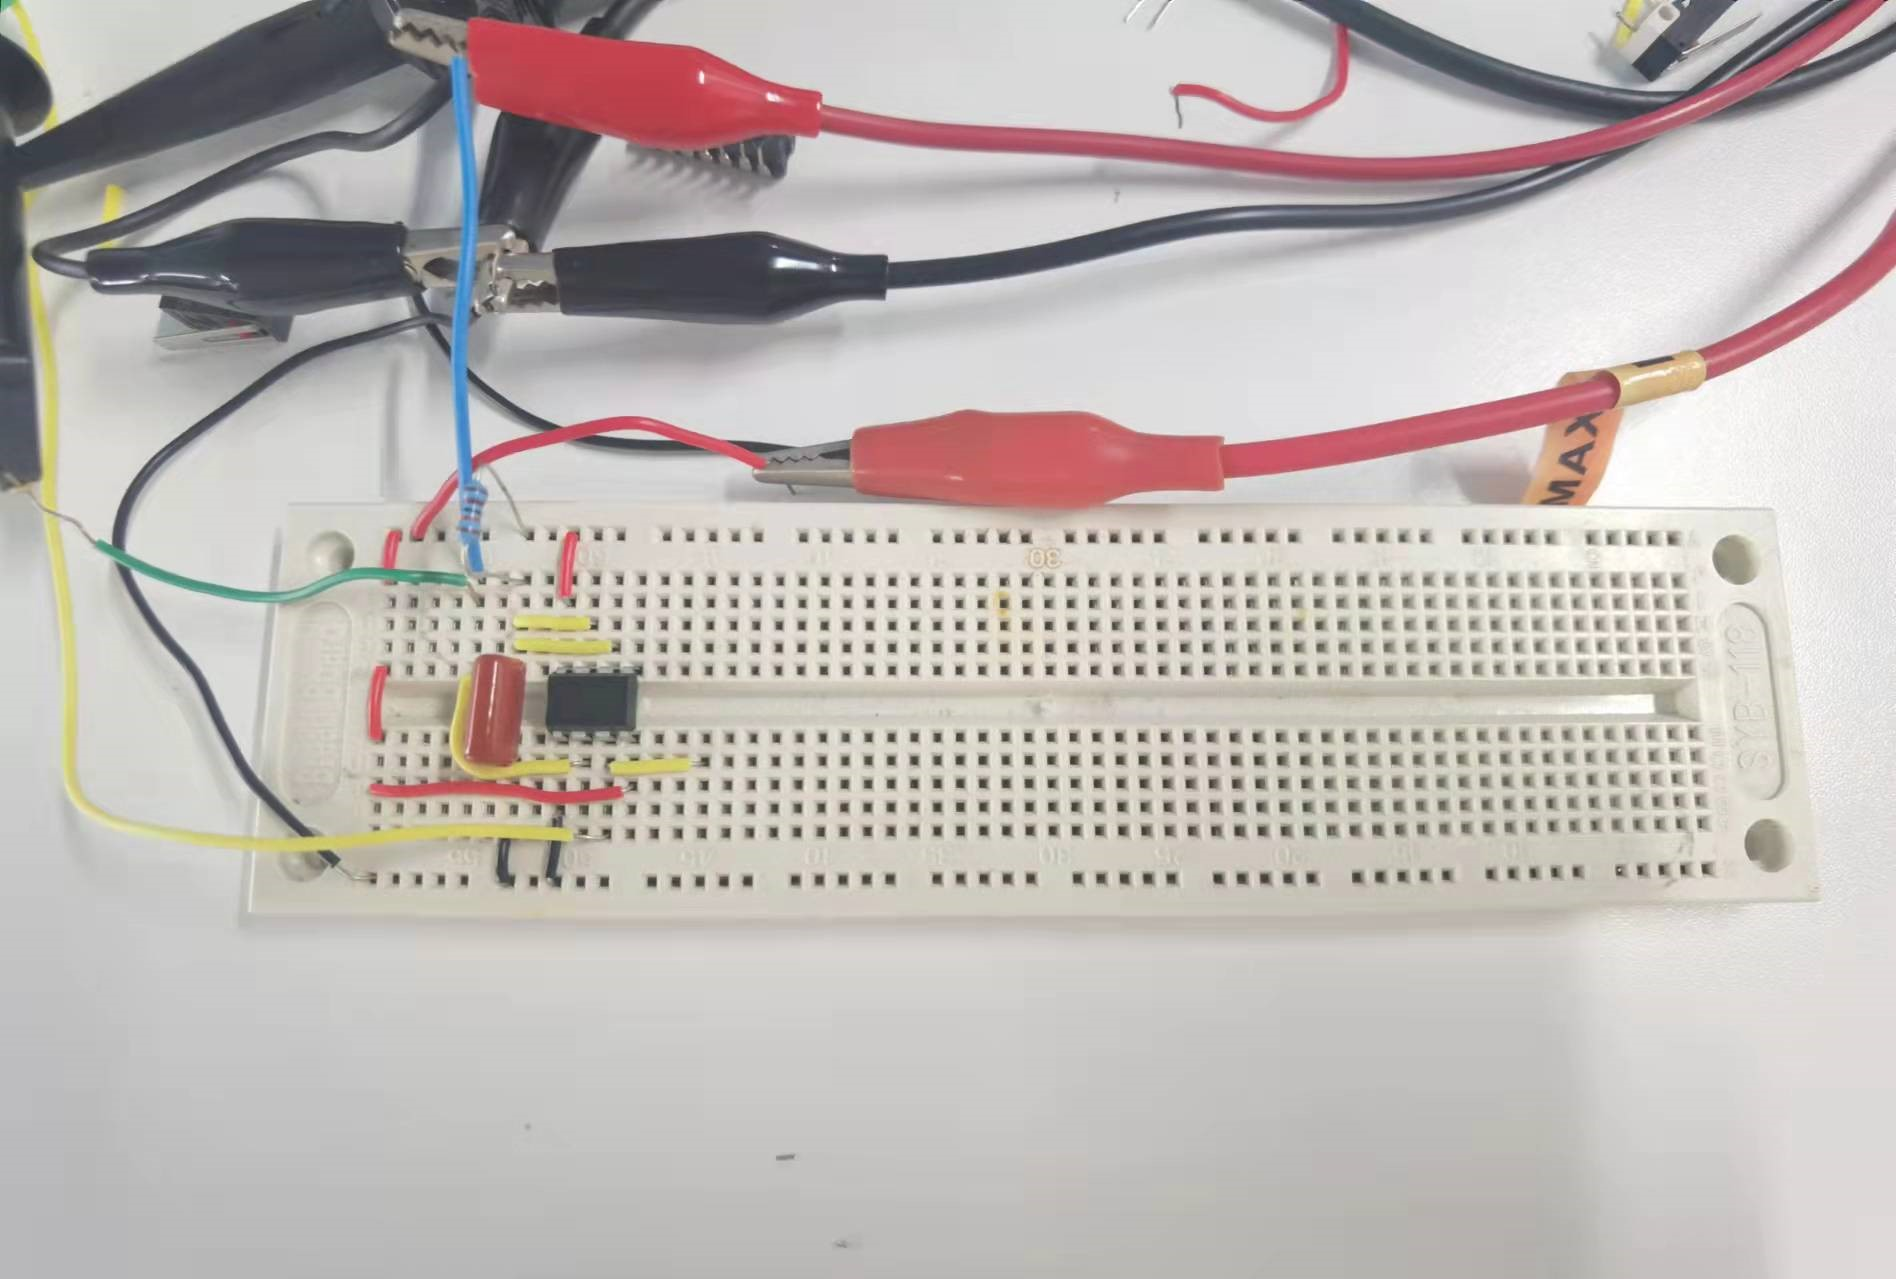
\includegraphics[width=0.8\textwidth]{555/monostable/circuit.jpg}
    \end{center}
    \caption{555单稳态触发器:实验电路}
    \label{monostable exp cir}
\end{figure}

\par 使用示波器观察引脚波形,其中通道1接\(V_{out}\),通道2接信号源信号。示波器波形如图\ref{monostable vout osci}所示。

\begin{figure}[H]
    \begin{center}
        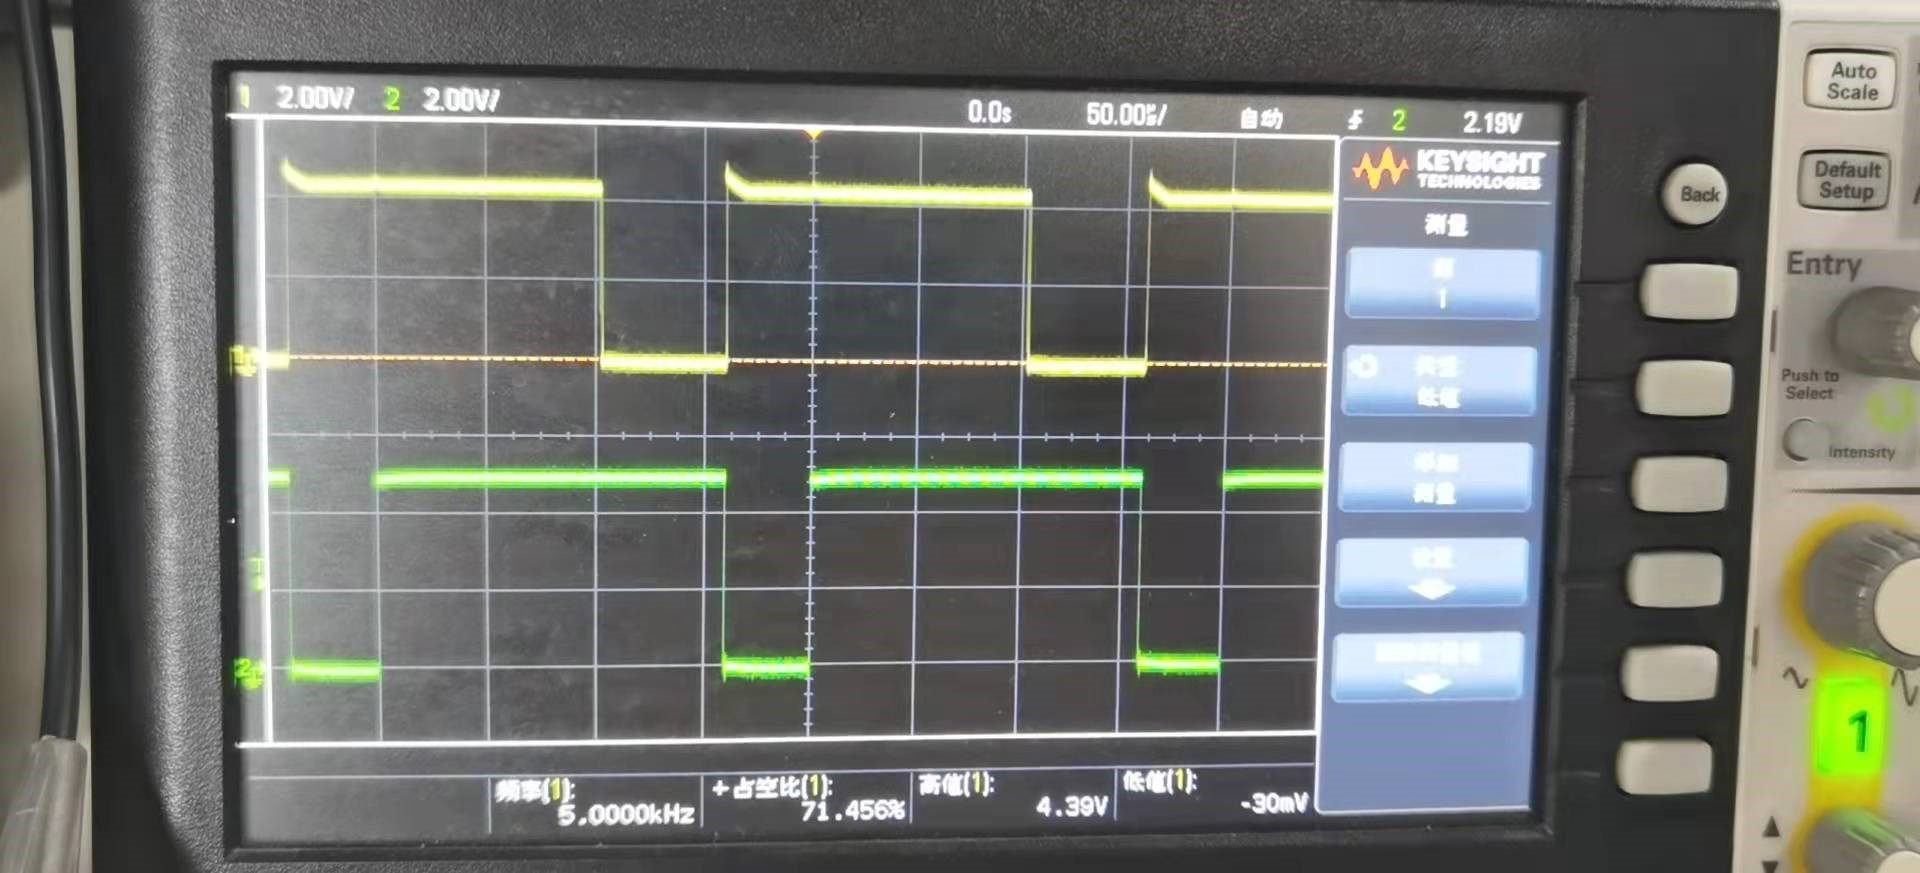
\includegraphics[width=0.8\textwidth]{555/monostable/vout.jpg}
    \end{center}
    \caption{555单稳态触发器:\(V_{out}\)波形}
    \label{monostable vout osci}
\end{figure}

测量得到信号\(V_{out}\)各参数如表\ref{monostable vout table}所示。

\begin{table}
    \begin{center}
        \begin{tabular}{c | c}
            物理量 & 值 \\
            \hline
            周期 & \SI{200}{\micro\second} \\
            高电平 & \SI{4.39}{\volt} \\
            低电平 & \SI{-30}{\milli\volt} \\
            高电平占空比 & 71.456\% \\
        \end{tabular}
        \label{monostable vout table}
        \caption{555单稳态触发器:\(V_{out}\)参数}
    \end{center}
\end{table}


\par 使用示波器观察引脚波形,其中通道1接\(V_c\),通道2接信号源信号。示波器波形如图\ref{monostable vc osci}所示。

\begin{figure}[H]
    \begin{center}
        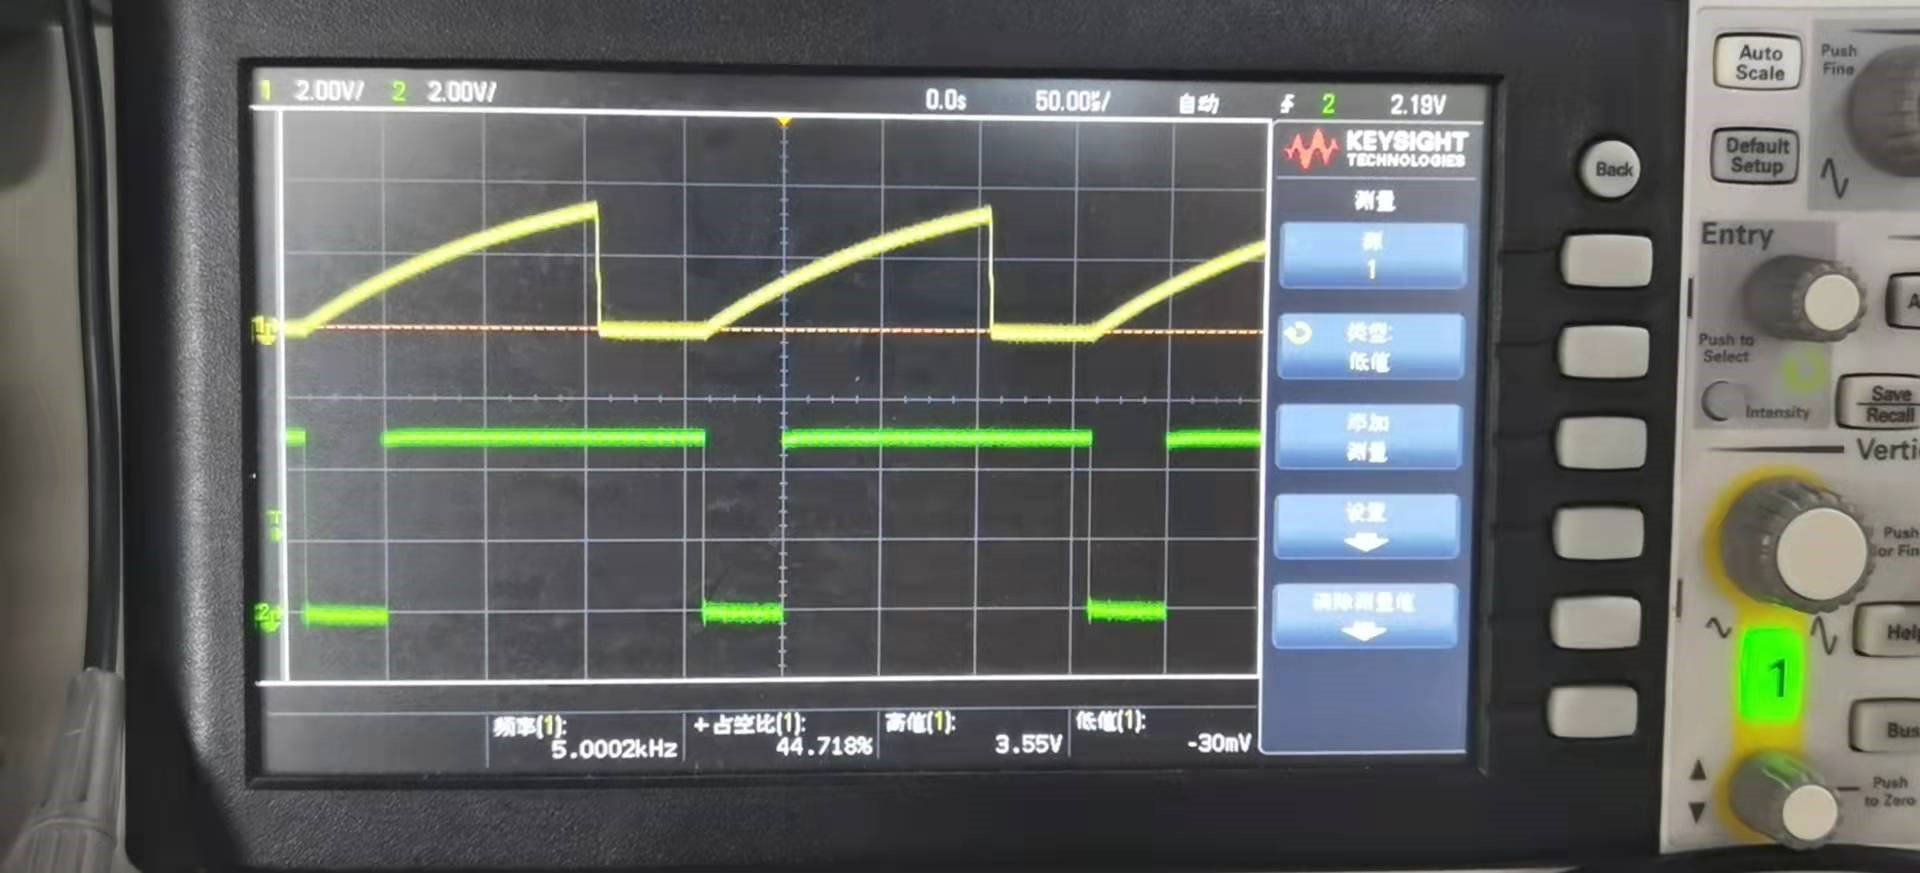
\includegraphics[width=0.8\textwidth]{555/monostable/vc.jpg}
    \end{center}
    \caption{555单稳态触发器:\(V_c\)波形}
    \label{monostable vc osci}
\end{figure}

测量得到信号\(V_c\)各参数如表\ref{monostable vc table}所示。

\begin{table}
    \begin{center}
        \begin{tabular}{c | c}
            物理量 & 值 \\
            \hline
            周期 & \SI{200}{\micro\second} \\
            高电平 & \SI{3.55}{\volt} \\
            低电平 & \SI{-30}{\milli\volt} \\
        \end{tabular}
        \label{monostable vc table}
        \caption{555单稳态触发器:\(V_c\)参数}
    \end{center}
\end{table}



\subsection{555定时器搭建多谐振荡器}
\subsubsection{原理电路}
\par 实验电路原理图如\ref{multiosci sim cir}所示,构成多谐振荡电路,TRI端低电平脉冲时触发输出高电平脉冲。对电路进行仿真,仿真结果如图\ref{multiosci sim res}所示。

\begin{figure}[H]
    \begin{center}
        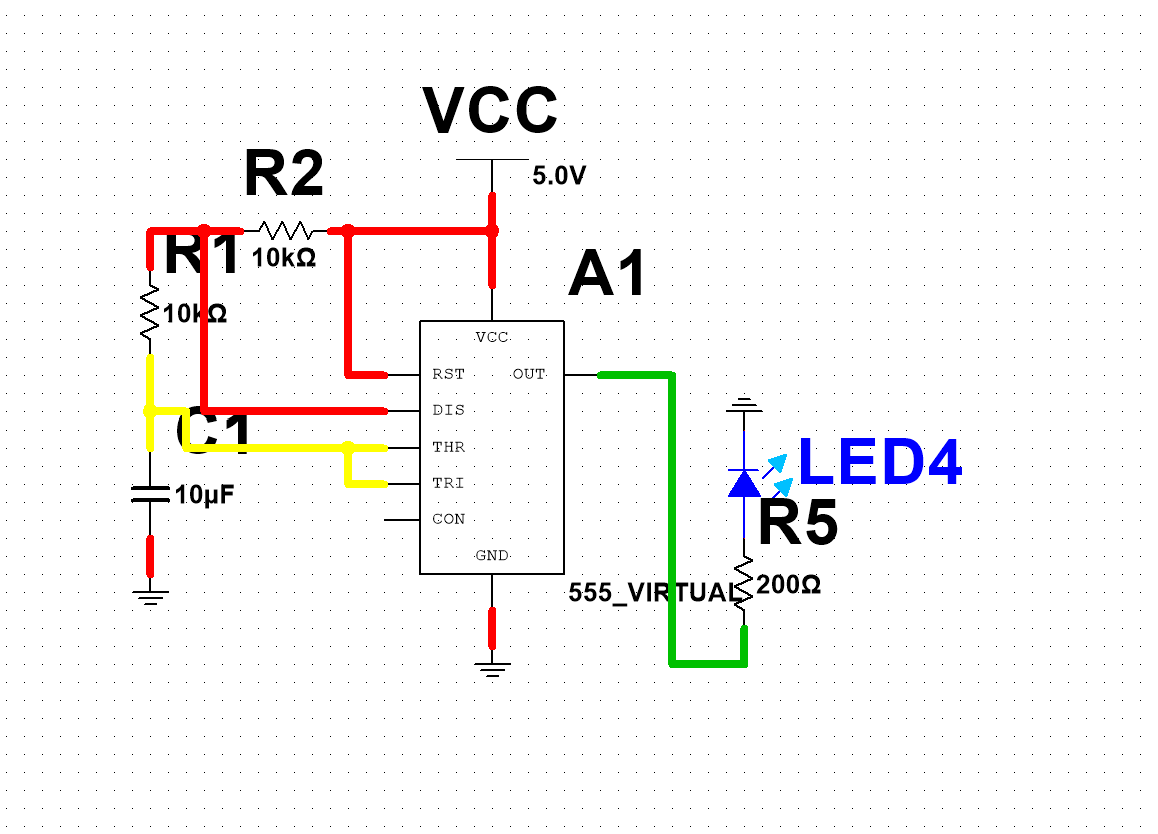
\includegraphics[width=0.8\textwidth]{555/multiosci/sim circuit.png}
    \end{center}
    \caption{555多谐振荡器:原理电路}
    \label{multiosci sim cir}
\end{figure}

\begin{figure}[H]
    \begin{center}
        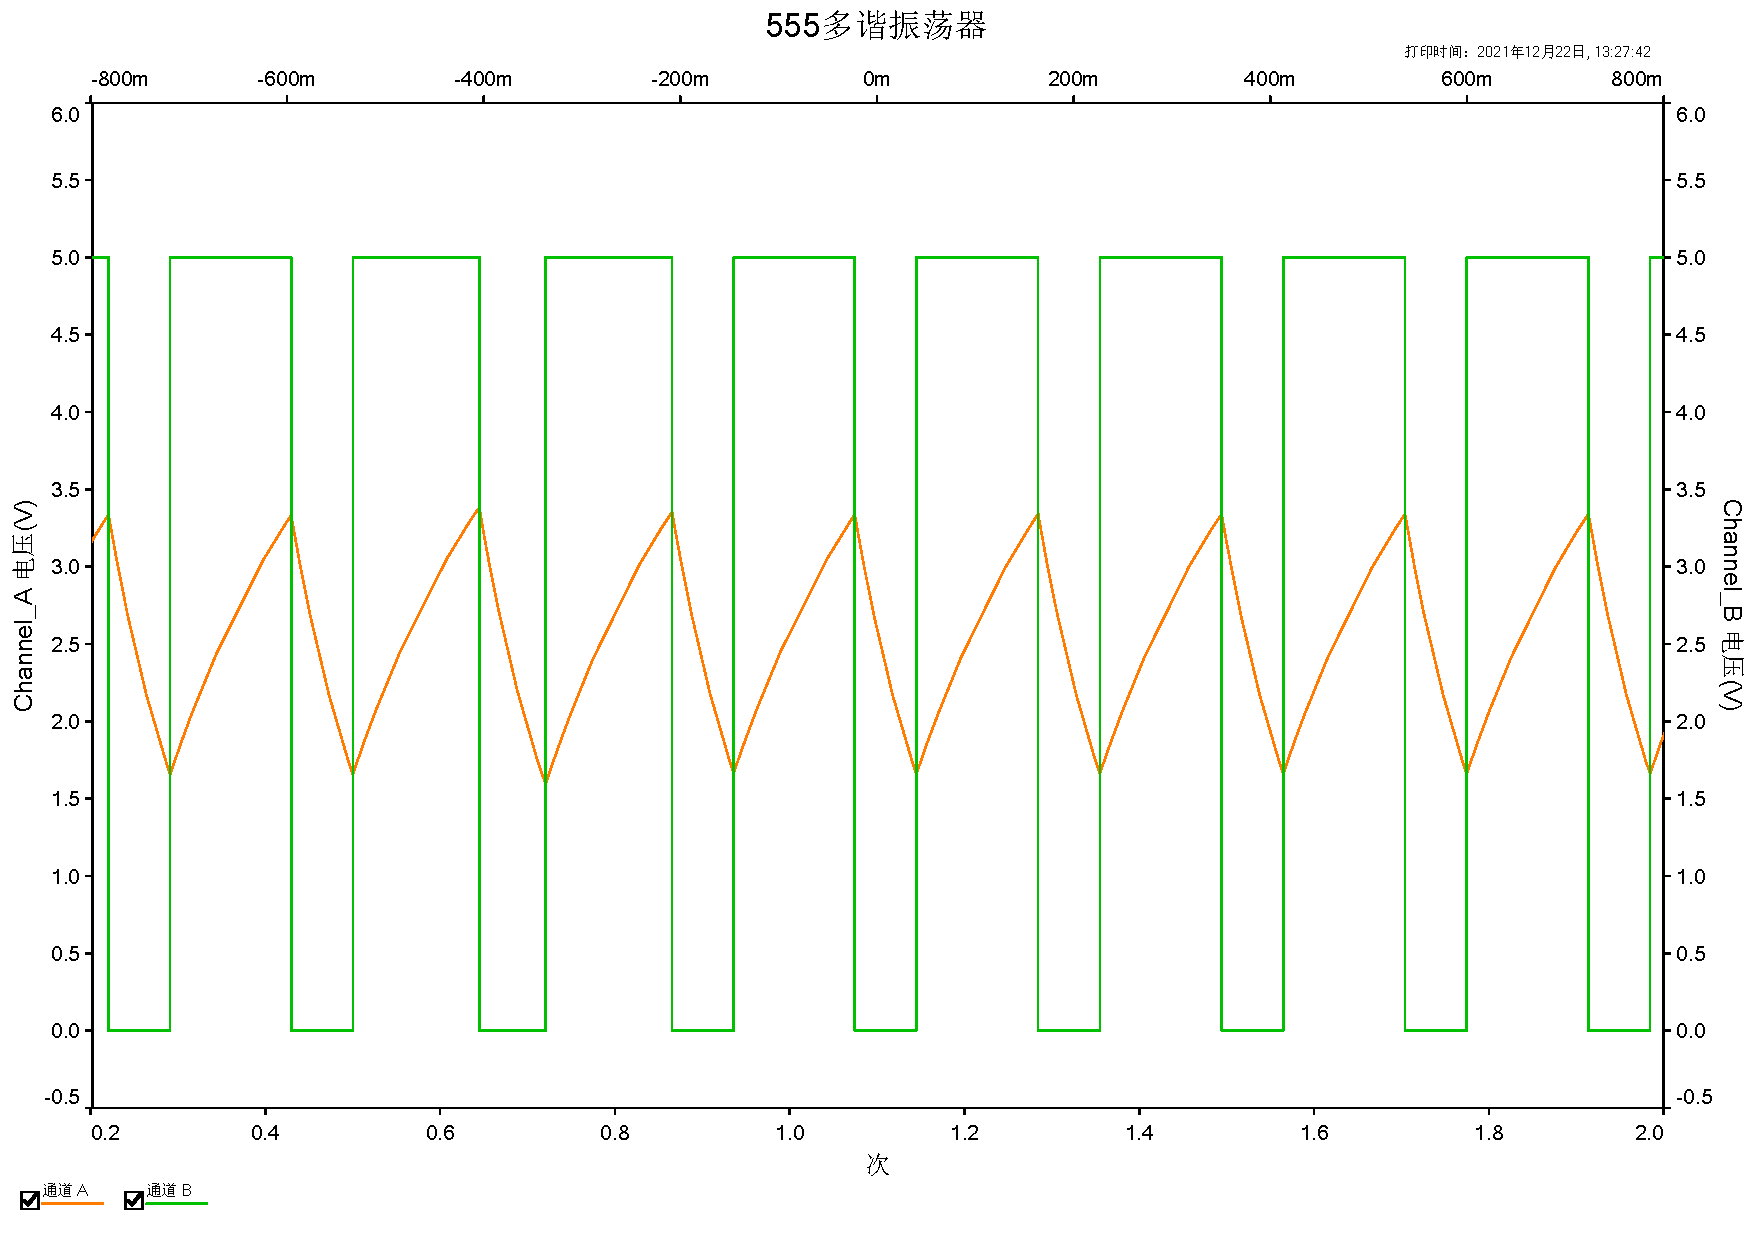
\includegraphics[width=0.8\textwidth]{555/multiosci/sim result.pdf}
    \end{center}
    \caption{555多谐振荡器:仿真波形}
    \label{multiosci sim res}
\end{figure}

\subsubsection{实验验证}
\par 按照原理电路中的电路连接、元件参数搭建实验电路,实验电路如图\ref{multiosci exp cir}所示。

\begin{figure}[H]
    \begin{center}
        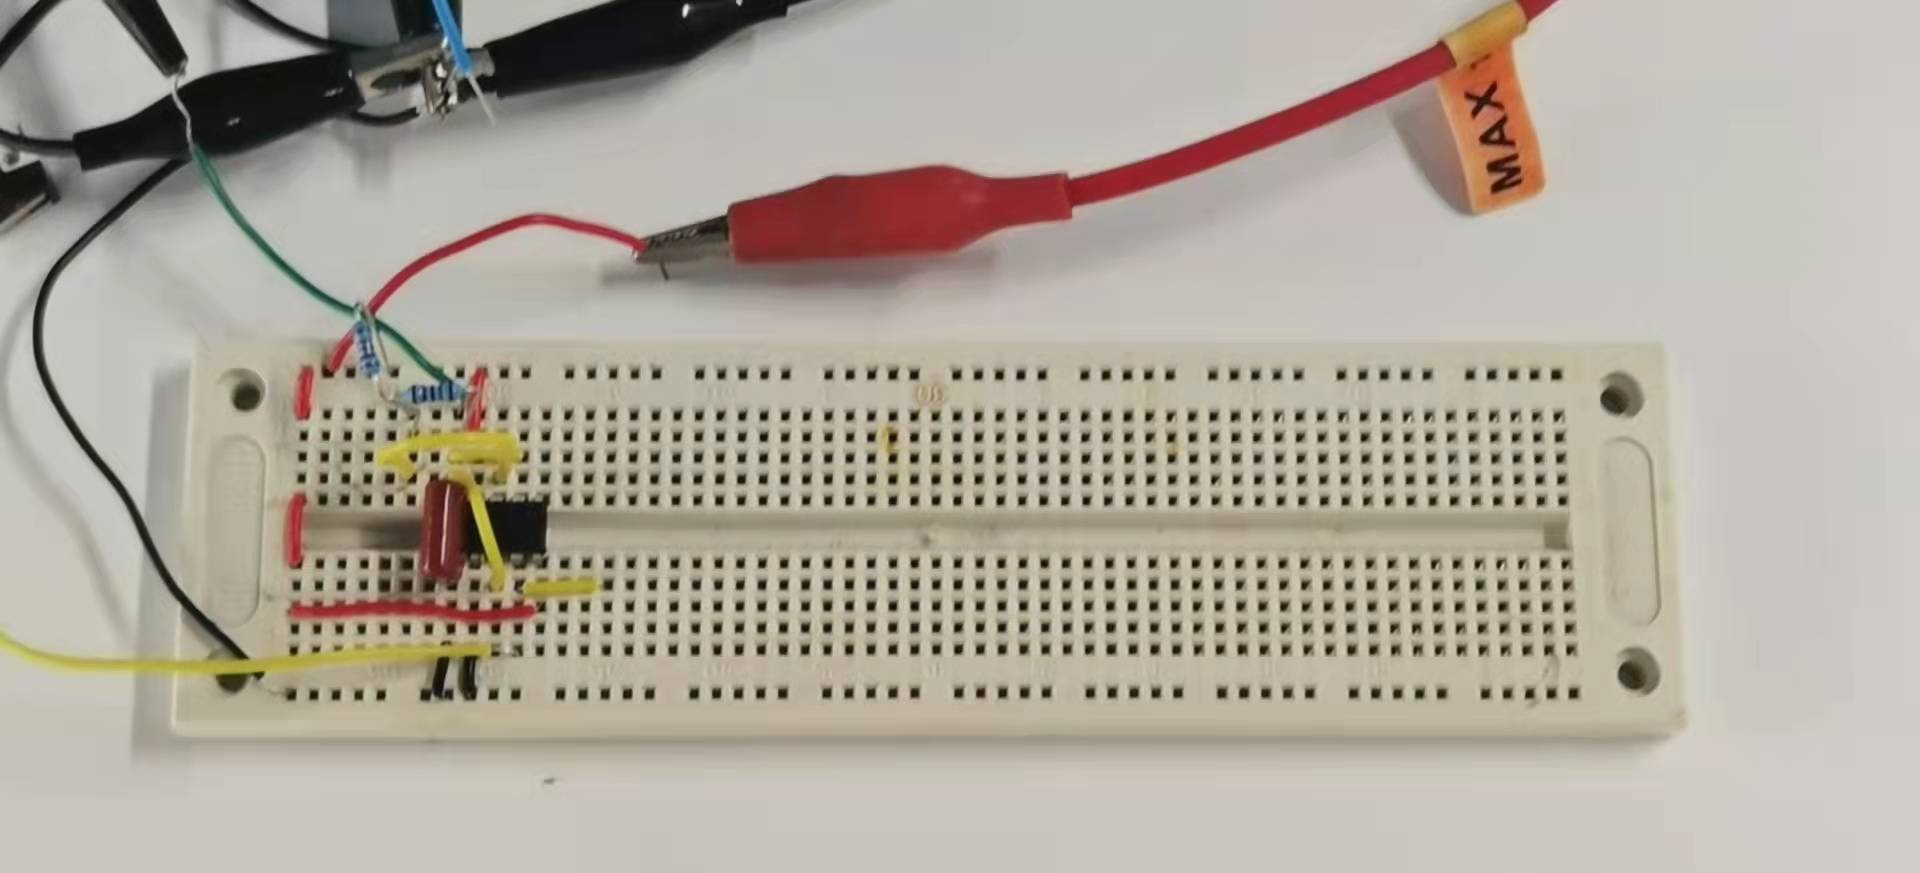
\includegraphics[width=0.8\textwidth]{555/multiosci/circuit.jpg}
    \end{center}
    \caption{555多谐振荡器:实验电路}
    \label{multiosci exp cir}
\end{figure}

\par 使用示波器观察引脚波形,其中通道1接\(V_{out}\),通道2接信号源信号。示波器波形如图\ref{multiosci vout osci}所示。

\begin{figure}[H]
    \begin{center}
        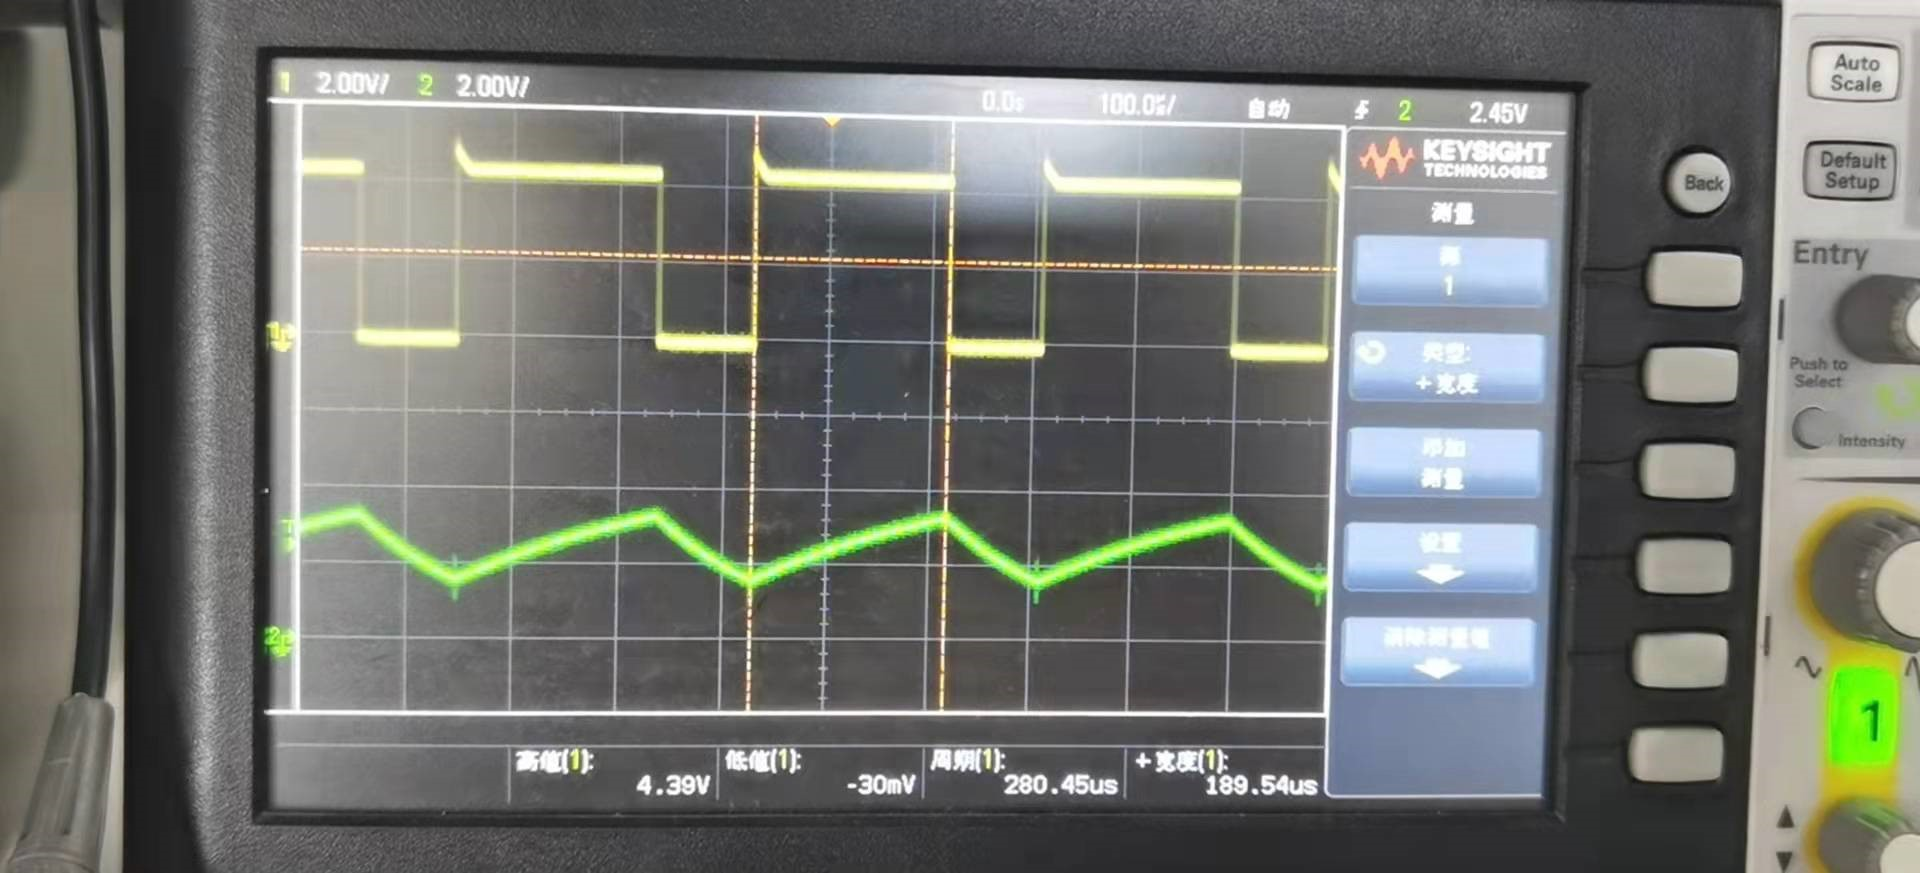
\includegraphics[width=0.8\textwidth]{555/multiosci/vout.jpg}
    \end{center}
    \caption{555多谐振荡器:\(V_{out}\)波形}
    \label{multiosci vout osci}
\end{figure}

测量得到信号\(V_{out}\)各参数如表\ref{multiosci vout table}所示。

\begin{table}
    \begin{center}
        \begin{tabular}{c | c}
            物理量 & 值 \\
            \hline
            周期 & \SI{280.45}{\micro\second} \\
            高电平宽度 & \SI{189.54}{\micro\second} \\
            高电平 & \SI{4.39}{\volt} \\
            低电平 & \SI{-30}{\milli\volt} \\
        \end{tabular}
        \label{multiosci vout table}
        \caption{555多谐振荡器:\(V_{out}\)参数}
    \end{center}
\end{table}


\par 使用示波器观察引脚波形,其中通道1接\(V_c\),通道2接信号源信号。示波器波形如图\ref{multiosci vc osci}所示。

\begin{figure}[H]
    \begin{center}
        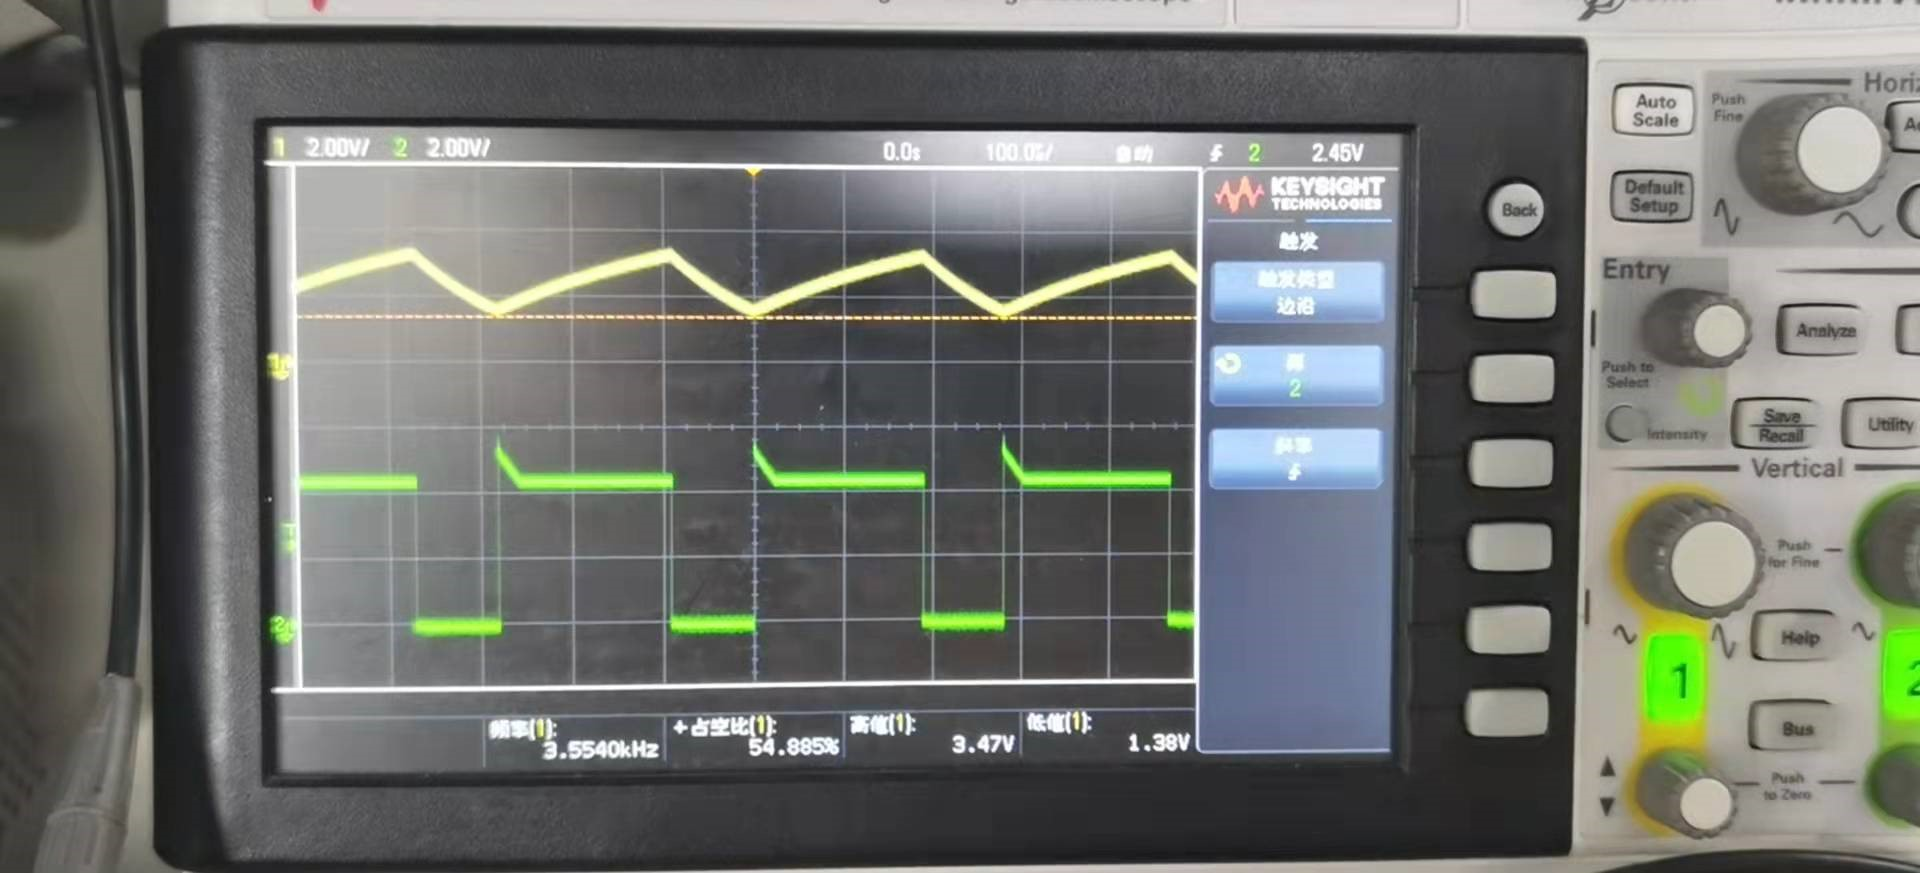
\includegraphics[width=0.8\textwidth]{555/multiosci/vc.jpg}
    \end{center}
    \caption{555多谐振荡器:\(V_c\)波形}
    \label{multiosci vc osci}
\end{figure}

测量得到信号\(V_c\)各参数如表\ref{multiosci vc table}所示。

\begin{table}
    \begin{center}
        \begin{tabular}{c | c}
            物理量 & 值 \\
            \hline
            周期 & \SI{280.45}{\micro\second} \\
            高电平 & \SI{3.47}{\volt} \\
            低电平 & \SI{1.38}{\volt} \\
        \end{tabular}
        \label{multiosci vc table}
        \caption{555多谐振荡器:\(V_c\)参数}
    \end{center}
\end{table}





\section{实验总结}

成功使用74LS90、74LS47以及数码管成功实现了十进制计数器、置零法以及置九法实现的六进制计数器、24进制计数器、38进制计数器。熟悉了使用硬件构建数字电路的操作,

\section*{原始数据}


\end{document}